\documentclass[10pt]{article}
\renewcommand{\baselinestretch}{1.8}

\usepackage[b4paper,left=0.8in,right=0.8in,top=0.8in,bottom=0.8in]{geometry}
\usepackage{tikz-qtree}
\usepackage{algorithm}
\usepackage{algpseudocode}
\makeatletter
\renewcommand{\ALG@beginalgorithmic}{\footnotesize}
\makeatother
\usepackage{graphicx}
\usepackage{subcaption}
\usepackage{showkeys}
\usepackage{amsmath}


\usepackage{multicol}
\setlength\columnsep{24pt}

\algnewcommand\algorithmicforeach{\bf{for each}}
\algdef{S}[FOR]{ForEach}[1]{\algorithmicforeach\ #1\ \algorithmicdo}

\algdef{S}[FUNCTION]{Function}
   [3]{{\tt{\sl{#1}}} \textproc{\tt{#2}}\ifthenelse{\equal{#3}{}}{}{\tt{(#3)}}}
  
\algdef{E}[FUNCTION]{EndFunction}
   [1]{\algorithmicend\ \tt{\textproc{#1}}}

\algrenewcommand\Call[2]{\tt{\textproc{#1}\ifthenelse{\equal{#2}{}}{}{(#2)}}}
   
\newcommand\keywordfont{\sffamily\bfseries}
\algrenewcommand\algorithmicend{{\keywordfont end}}
\algrenewcommand\algorithmicfor{{\keywordfont for}}
\algrenewcommand\algorithmicforeach{{\keywordfont for each}}
\algrenewcommand\algorithmicdo{{\keywordfont do}}
\algrenewcommand\algorithmicuntil{{\keywordfont until}}
\algrenewcommand\algorithmicfunction{{\keywordfont function}}
\algrenewcommand\algorithmicif{{\keywordfont if}}
\algrenewcommand\algorithmicthen{{\keywordfont then}}
\algrenewcommand\algorithmicelse{{\keywordfont else}}
\algrenewcommand\algorithmicreturn{{\keywordfont return}}

\renewcommand\thealgorithm{}
\newcommand{\setalglineno}[1]{%
  \setcounter{ALC@line}{\numexpr#1-1}}

\newcommand{\sub}[1]{\textsubscript{#1}}
\renewcommand{\tt}[1]{\texttt{#1}}
\renewcommand{\sl}[1]{\textsl{#1}}
\renewcommand{\it}[1]{\textit{#1}}
\renewcommand{\bf}[1]{\textbf{#1}}
\newcommand{\nf}[1]{\normalfont{#1}}
\newcommand{\cmt}[1]{\Comment{#1}}

\usepackage{amsmath,amssymb,amsthm}
\newtheorem{theorem}{Theorem}
\newtheorem{lemma}[theorem]{Lemma}
\theoremstyle{definition}
\newtheorem{definition}[theorem]{Definition}

\begin{document}

\section{Pseudocode}

\begin{algorithm}
\caption{Fields description}
\begin{algorithmic}[1]
\setcounter{ALG@line}{100}
\begin{multicols}{2}

\Statex \bf{Structure}

\Statex $\diamondsuit$ \tt{\sl{Shared}}
\begin{itemize}
\item \tt{\sl{Tree} tree} \textsf{: A binary tree of \tt{Node}s. \tt{root} is a pointer to the root node.}
%such that \tt{root} is the root and the left child and the right child and the parent of \tt{Tree[i]} are \tt{Tree[2i+1]}, \tt{Tree[2i+2]} and \tt{Tree[i/2]}.
\end{itemize}

\Statex

\Statex $\diamondsuit$ \tt{\sl{Local}}
\begin{itemize}
\item \tt{\sl{*Node} leaf:} \sf{ a pointer to the process's leaf in the tree.}
\end{itemize}

\Statex
\Statex $\diamondsuit$ \tt{\sl{Structures}}

\Statex $\blacktriangleright$ \tt{\sl{Node}}
\begin{itemize}
\item \tt{\sl{*Node} left, right, parent} \textsf{: initialized  when creating the tree.}
\item \tt{\sl{BlockList} blocks}
  \textsf{ implemented with an array.}
\item \tt{\sl{int} size= 1}\textsf{: \#\tt{block}s in \tt{blocks}.}
\item \tt{\sl{int} num\sub{propagated}= 0}\textsf{} \textsf{: \# groups of blocks that have been propagated from the node to its parent. Since it is incremented after propagating, it may be behind by 1.}
\item \tt{\sl{int[]} super}\textsf{: \tt{super[i]} stores an approximate index of the superblock of the blocks in \tt{blocks} whose \tt{group} field have value \tt{i}.}
\end{itemize}

%\Statex $\blacktriangleright$ \tt{\sl{Root} extends \sl{Node}}
%\begin{itemize}
%  
%\item \tt{\sl{PBRT} blocks}
%
%  \textsf{\tt{BlockList} is implemented with a persistent red-black tree.}
%  
%\end{itemize}

%\Statex $\blacktriangleright$ \tt{\sl{NonRootNode} extends \sl{Node}}
%\begin{itemize}
    
%\end{itemize}

\Statex $\blacktriangleright$ \tt{\sl{Leaf} extends \sl{NonRootNode}}
\begin{itemize}
  
  \item \tt{\sl{int} \tt{last\sub{done}}}

  \textsf{Stores the index of the block in the root such that the process that owns this leaf has most recently finished the. A block is finished if all of its operations are finished. \tt{enqueue(e)} is finished if \tt{e} is returned by some \tt{dequeue()} and \tt{dequeue()} is finished when it computes its response. \it{put the definitions before the pseudocode}}
  
\end{itemize}
\pagebreak

\Statex $\blacktriangleright$ \tt{\sl{Block}} 
%\cmt{If \tt{b} is \tt{blocks[i](i!=0)} then \tt{b[-1] is blocks[i-1].}}
\cmt{For a \tt{block} in a \tt{blocklist} we define \it{the prefix for the block} to be the blocks in the \tt{BlockList} up to and including the \tt{block}. \it{put the definitions before the pseudocode}}

\begin{itemize}
%  \item \tt{\sl{int} num\sub{enq}, num\sub{deq}}
%  \textsf{: \# enqueue, dequeue operations in the block}
%  \item \tt{\sl{int} num, sum}
%  \textsf{: total \# operations in block, prefix sum of \tt{num}}

  \item \tt{\sl{int} group}
  \textsf{: the value read from \tt{num\sub{propagated}} when appending this block to the node.}
\end{itemize}


\Statex $\blacktriangleright$ \tt{\sl{LeafBlock} extends \sl{Block}}
\begin{itemize}
  \item \tt{\sl{Object} element}
  \textsf{: Each block in a leaf represents a single operation. For \tt{enqueue} operations element is the input of the \tt{enqueue} and for \tt{dequeue} operations it is \tt{null}.}
  
    \item \tt{\sl{Object} response}
  \textsf{: stores the response of the operation in the \tt{LeafBlock}.}
  
    \item \tt{\sl{int} sum\sub{enq}, sum\sub{deq}}
  \textsf{: \# enqueue, dequeue operations in the prefix for the block}
  
\end{itemize}

\Statex $\blacktriangleright$ \tt{\sl{InternalBlock} extends \sl{Block}}
\begin{itemize}
    \item \tt{\sl{int} end\sub{left}, end\sub{right}}
  \textsf{:~~index of the last subblock of the block in the left and right child}
  \item \tt{\sl{int} sum\sub{enq-left}}
  \textsf{: \# enqueue operations in the prefix for \tt{left.blocks[end\sub{left}]}}
  \item \tt{\sl{int} sum\sub{deq-left}}
  \textsf{: \# dequeue operations in the prefix for \tt{left.blocks[end\sub{left}]}}
  \item \tt{\sl{int} sum\sub{enq-right}}
  \textsf{: \# enqueue operations in the prefix for \tt{right.blocks[end\sub{right}]}}
  \item \tt{\sl{int} sum\sub{deq-right}}
  \textsf{: \# dequeue operations in the prefix for \tt{right.blocks[end\sub{right}]}}
\end{itemize}


\Statex $\blacktriangleright$ \tt{\sl{RootBlock} extends \sl{InternalBlock}}
\begin{itemize}
  \item \tt{\sl{int} length}
  \textsf{: length of the queue after performing all operations in the prefix for this block}
%  \item \tt{\sl{int} sum\sub{non-null deq}}
%  \textsf{: count of non-null dequeus up to this block}
  \item \tt{\sl{counter} num\sub{finished}}
  \textsf{: number of finished operations in the block}
    \item \tt{\sl{int} order}
  \textsf{: the index of the block in the \tt{BlockList} containing the block.}
\end{itemize}

%\Statex $\blacktriangleright$ \tt{Conventions}
%\begin{itemize}
%  \item \tt{i} : index of ith operation in the tree
%  \item \tt{j} : index of jth operation in a node
%  \item \tt{b\sub{n}} : index of the block containing the operation n based on the scope
%  \item Also we are not going to refer to blocks directly, only with their indices. Except while constructing a new block.
%\end{itemize}


\end{multicols}
\end{algorithmic}
\end{algorithm}


\begin{footnotesize}
  
\it{Variable naming:}
\begin{itemize}
  \item \tt{b\sub{op}}: index of the block containing operation\tt{op}
  \item \tt{r\sub{op}}: rank of operation \tt{op} i.e. the ordering among the operations of its type according to linearization ordering
\end{itemize}

\it{Abbreviations:}
\begin{itemize}
 \item \tt{blocks[b].sum\sub{x}=blocks[b].sum\sub{x-left}+blocks[b].sum\sub{x-right}}  \tt{ (for b$\geq$0 and x $\in$ \{enq, deq\}})
 \item \tt{blocks[b].sum=blocks[b].sum\sub{enq}+blocks[b].sum\sub{deq}}  \tt{ (for b$\geq$0})
  \item \tt{blocks[b].num\sub{x}=blocks[b].sum\sub{x}-blocks[b-1].sum\sub{x}} \\ \tt{(for b>0 and x $\in$ \{$\emptyset$, enq, deq, enq-left, enq-right, deq-left, deq-right\}, blocks[0].num\sub{x}=0})
\end{itemize}
\end{footnotesize}



%##########################################


\begin{algorithm}
\caption{\tt{\sl{Queue}}}
\begin{algorithmic}[1]
\setcounter{ALG@line}{200}
\begin{multicols}{2}

\Function{void}{Enqueue}{\sl{Object} e} \cmt{Creates a block with element \tt{e} and appends it to the tree.}
\State \tt{block newBlock= \Call{new}{\sl{LeafBlock}}}
\State \tt{newBlock.element= e}
%\State \tt{b.num\sub{enq}=1}
\State \tt{newBlock.sum\sub{enq}= leaf.blocks[leaf.size].sum\sub{enq}+1}
\State \tt{newBlock.sum\sub{deq}= leaf.blocks[leaf.size].sum\sub{deq}}
\State \tt{leaf.}\Call{Append}{newBlock}
\EndFunction{Enqueue}

\Statex
\Function{Object}{Dequeue()}{}
\State \tt{block newBlock= \Call{new}{\sl{LeafBlock}}} \cmt{Creates a block with null value element, appends it to the tree, computes its order among operations, then computes and returns its response.}
\State \tt{newBlock.element= null}
\State \tt{newBlock.sum\sub{enq}= leaf.blocks[leaf.size].sum\sub{enq}}
\State \tt{newBlock.sum\sub{deq}= leaf.blocks[leaf.size].sum\sub{deq}+1}
\State \tt{leaf.}\Call{Append}{newBlock}
\State \Return\tt{leaf.}\Call{HelpDequeue()}{}
\EndFunction{Dequeue}

\Statex
\pagebreak

\Function{int, int}{FindResponse}{int i, int b}\cmt{Computes the rank  and index of the block in the root of the enqueue that is the response of the \tt{i}th dequeue in the root's \tt{b}th block. Returns \tt{<-1,-->} if the queue is empty.}
\If{\tt{root.blocks[b-1].length + root.blocks[b].num\sub{enq} - i $<$ 0}}
\State \Return \tt{<-1,-->}
\Else
\Statex \cmt{We call the dequeues that return a value \it{non-null dequeues}. $r$th non-null dequeue returns the element of th $r$th enqueue. We can compute \# non-null dequeues in the prefix for a block this way: \#non-null dequeues= length - \#enqueues. Note that the $i$th dequeue in the given block is not a non-null dequeue.}
\State \tt{r\sub{enq}= root.blocks[b-1].sum\sub{enq}- root.blocks[b-1].length + i}
\State \Return \tt{<root.blocks.get(enq, r\sub{enq}).order, r\sub{enq}>}
\EndIf
\EndFunction{FindResponse}

\end{multicols}
\end{algorithmic}
\end{algorithm}


%##########################################


\begin{algorithm}
\caption{\tt{\sl{Node}}}
\begin{algorithmic}[1]
\setcounter{ALG@line}{300}
\begin{multicols}{2}

\Function{void}{Propagate()}{}
\If{\bf{not} \Call{Refresh()}{}}
\State \Call{Refresh()}{} \cmt{Lemma Double Refresh}
\EndIf
\If{\tt{this} \bf{is not} \tt{root}}
\State \tt{parent.}\Call{Propagate()}{}
\EndIf
\EndFunction{Propagate}

\Statex

\Function{boolean}{Refresh()}{}
\State \tt{s= size}
%\If{\tt{n.blocks[h]!=null?}} \tt{h+=1}\EndIf
\State \tt{<new, np\sub{left}, np\sub{right}>= \Call{CreateBlock}{h}} \cmt{\tt{np\sub{left}, np\sub{right}} are the values read from the children's \tt{num\sub{propagated}} feild.}
\If{\tt{new.num==0}} \Return{\tt{true}} \cmt{The block contains nothing.}
\ElsIf{\tt{blocks.tryAppend(new, s)}}
\ForEach{\tt{dir} {\keywordfont{in}} \tt{\{left, right\}}} \label{okcas}
\State \tt{\Call{CAS}{dir.super[np\sub{dir}], null, h+1}} \cmt{Write would work too.}
\State \tt{\Call{CAS}{dir.num\sub{propagated}, np\sub{dir}, np\sub{dir}+1}}
\EndFor
\State \tt{\Call{CAS}{size, h, h+1}}
\State \Return{\tt{true}}
\Else
\State \tt{\Call{CAS}{size, h, h+1}} \cmt{Even if another process wins, help to increase the size. The winner might have fallen sleep before increasing \tt{size}.}
\State \Return{ \tt{false}}
\EndIf
\EndFunction{Refresh}

\Statex

\Statex $\leadsto$ \textsf{Precondition: \tt{blocks[start..end]} contains a block with field \tt{f} $\geq$ \tt{i}}
\Function{int}{BSearch}{\sl{field} f, \sl{int} i, \sl{int} start, \sl{int} end}

\Statex \cmt{\textmd{Does binary search for~the value \tt{i} of the given prefix sum \tt{field}. Returns the index of the leftmost block in \tt{blocks[start..end]} whose \sl{field} \tt{f} is $\geq$ \tt{i}}.}
%\State \Return \tt{result block's index}
\EndFunction{BSearch}

\pagebreak

\Function{<Block, int, int>}{CreateBlock}{\sl{int} i} 
\Statex\cmt{Creates a block to be inserted into as $i$th \tt{block} in \tt{blocks}. Returns the created block as well as values read from each child's num\sub{propagated} field. These values are used for incrementing the children's num\sub{propagated} field if the block was appended to \tt{blocks} successfully.}
\State \tt{block newBlock= \Call{new}{\sl{block}}}
\State \tt{newBlock.group= num\sub{propagated}}
\State \tt{newBlock.order= i}
\ForEach{\tt{dir} {\keywordfont{in}} \tt{\{left, right\}}}
\State \tt{index\sub{last}= dir.size} \label{lastLine}
\State \tt{index\sub{prev}= blocks[i-1].end\sub{dir}} \label{prevLine}
\State \tt{newBlock.end\sub{dir}= index\sub{last}}
\State \tt{block\sub{last}= dir.blocks[index\sub{last}]}
\State \tt{block\sub{prev}= dir.blocks[index\sub{prev}]}
\State \cmt{\tt{newBlock} includes \tt{dir.blocks[index\sub{prev}+1..index\sub{last}]}.}
\State \tt{this\sub{dir}= dir.num\sub{propagated}}
\State \tt{newBlock.sum\sub{enq-dir}= blocks[i-1].sum\sub{enq-dir} + block\sub{last}.sum\sub{enq} - block\sub{prev}.sum\sub{enq}}
\State \tt{newBlock.sum\sub{deq-dir}= blocks[i-1].sum\sub{deq-dir} + block\sub{last}.sum\sub{deq} - block\sub{prev}.sum\sub{deq}}
\EndFor
%\State \tt{b.num\sub{enq}= b.num\sub{enq-left} + b.num\sub{enq-right}}
%\State \tt{b.num\sub{deq}= b.num\sub{deq-left} + b.num\sub{deq-right}}
%\State \tt{b.num= b.num\sub{enq} + b.num\sub{deq}}
%\State \tt{b.sum= n.blocks[i-1].sum + b.num}

\If{\tt{this} \bf{is} \tt{root}}
\State \tt{newBlock.length= max(root.blocks[i-1].length + b.num\sub{enq} - b.num\sub{deq}, 0)}
%\State \tt{b.sum\sub{non-null deq}= root.blocks[i-1].sum\sub{non-null deq} + max( b.num\sub{deq} - root.blocks[i-1].length - b.num\sub{enq}, 0)}
\EndIf

\State \Return \tt{<b, np\sub{left}, np\sub{right}>}
\EndFunction{CreateBlock}

\end{multicols}
\end{algorithmic}
\end{algorithm}

%##########################################

\begin{algorithm}
\caption{Node}
\begin{algorithmic}[1]
\setcounter{ALG@line}{400}

\Statex $\leadsto$ \textsf{Precondition:~\tt{blocks[b].num\sub{enq}$\geq$i}}
\Function{element}{GetEnq}{\sl{int} b, \sl{int} i} 
\If{\tt{this} \bf{is} \tt{leaf}}
\State\Return \tt{blocks[b].element}
\ElsIf{\tt{i $\leq$ blocks[b].num\sub{enq-left}}} \cmt{\tt{i} exists in the left child of this node}
\State \tt{subBlock= left.\Call{BSearch}{sum\sub{enq}, i, blocks[b-1].end\sub{left}+1, blocks[b].end\sub{left}}} \cmt{Search range of left child's subblocks of \tt{blocks[b]}.}
\State \Return\tt{left.}\Call{Get}{i-left.blocks[subBlock-1].sum\sub{enq}, subBlock} 
\Else
\State \tt{i= i-blocks[b].num\sub{enq-left}}
\State\tt{subBlock= right.\Call{BSearch}{sum\sub{enq}, i, blocks[b-1].end\sub{right}+1, blocks[b].end\sub{right}}} \cmt{Search range of right child's subblocks of \tt{blocks[b]}.}
\State \Return\tt{right.}\Call{Get}{i-right.blocks[subBlock-1].sum\sub{enq}, subBlock} 
\EndIf
\EndFunction{GetEnq}

\Statex
\Statex $\leadsto$ \textsf{Precondition: \tt{b}th block of the node has propagated up to the root and \tt{blocks[b].num\sub{enq}$\geq$i}.}
\Function{<int, int>}{IndexDeq}{\sl{int} b, \sl{int} i} \cmt{Returns the rank of $i$th dequeue in the $b$th block of the node, among the dequeues in the root.}
\If{\tt{this} \bf{is} \tt{root}}
\State\Return \tt{<b, i>}
\Else
\State \tt{dir= (parent.left==n)? left: right} \cmt{check if a left or a right child}
\State \tt{superBlock= parent.\Call{BSearch}{sum\sub{deq-dir}, i, super[blocks[b].group]-p, super[blocks[b].group]+p}} 
\Statex\cmt{superblock's group has at most $p$ difference with the value stored in \tt{super[]}.}
\If{\tt{dir {\keywordfont is} right}}
%\State \tt{i+= parent.blocks[superBlock-1].sum\sub{deq-right}}
\State \tt{i+= blocks[superBlock].sum\sub{deq-left}} \cmt{consider the dequeues from the right child}
\EndIf
\State \Return\tt{this.parent.}\Call{IndexDeq}{superBlock, i}
\EndIf
\EndFunction{Index}

\end{algorithmic}
\end{algorithm}


%##########################################

\begin{algorithm}
\caption{Leaf}
\begin{algorithmic}[1]
\setcounter{ALG@line}{500}

\Function{void}{Append}{\sl{block} blk} \cmt{Append is only called by the owner of the leaf.}
\State \tt{size+=1} \label{appendEnd} 
\State \tt{blk.group= size} \label{appendStart} 
\State \tt{blocks[size]= blk} 
\State \tt{parent.}\Call{Propagate()}{} 
\EndFunction{Append}

\Statex

\Function{Object}{HelpDequeue()}{}
\State \tt{<b\sub{deq}, r\sub{deq}>=} \Call{IndexDeq}{leaf.size, 1}\cmt{\tt{r} is the rank among the dequeues of the dequeue of  the \tt{b\sub{deq}}th block in the root containing.}
\State \tt{<r\sub{enq}, r\sub{enq}>=} \Call{FindResponse}{r\sub{deq}, b\sub{deq}} 
 \cmt{\tt{r\sub{enq}} is the rank of the enqueue whose element is the response to the dequeue in the block containing it and \tt{b\sub{deq}} is the index of that block of it in the blocklist. If the response is \tt{null} then r\sub{deq} is -1.} \label{deqRest}
\If{\tt{r\sub{enq}==-1}}
\State \tt{output= null}
\State \tt{root.blocks[b\sub{deq}].num\sub{finished}.inc()} \cmt{shared counter}
\If{\tt{root.blocks[b\sub{deq}].num\sub{finished}==root.blocks[b\sub{deq}].num}}
\State \tt{last\sub{done}= b\sub{deq}}
\EndIf
\pagebreak
\Else
\State \tt{output= \Call{GetEnq}{b\sub{enq}, r\sub{enq}}} \cmt{getting the reponse's \tt{element}.}
\State \tt{root.blocks[b\sub{enq}].num\sub{finished}.inc()}
\State \tt{root.blocks[b\sub{enq}].num\sub{finished}.inc()}
\If{\tt{root.blocks[b\sub{deq}].num\sub{finished}==root.blocks[b\sub{deq}].num}} 
\State \tt{last\sub{done}= b\sub{deq}}
\ElsIf{\tt{root.blocks[b\sub{enq}].num\sub{finished}==root.blocks[b\sub{enq}].num}}
\State \tt{last\sub{done}= b\sub{enq}}
\EndIf
\EndIf
\State \Return{\tt{output}}
\EndFunction{Dequeue}


\end{algorithmic}
\end{algorithm}


%##########################################

\begin{algorithm}
\caption{BlockList}
\begin{algorithmic}[1]
\setcounter{ALG@line}{600}

\Statex \cmt{\textsf{: Supports two operations \tt{blocks.tryAppend(Block b), blocks[i]}. Initially  empty, when \tt{blocks.tryAppend(b, n)} returns true \tt{b} is appended to \tt{blocks[n]} and \tt{blocks[i]} returns $i$th block in the \tt{blocks}. If some instance of \tt{blocks.tryAppend(b, n)} returns \tt{false} there is a concurrent instance of \tt{blocks.tryAppend(b$^\prime$, n)} which has returned \tt{true}.\tt{blocks[0]} contains an empty block with all fields equal to 0 and \tt{end\sub{left}, end\sub{right}} pointers to the first block of the corresponding children.}}

\Statex
\Statex $\diamondsuit$ \tt{\sl{PBRT implementation}}
  \Statex \sf{A persistant red-black tree supporting \tt{append(b, key),get(key=i),split(j)}}.
  \tt{append(b, key) returns \tt{true} in case successful. Since \tt{order, sum\sub{enq}}are both strictly increasing we can use one of them for another.}
\Statex \tt{root: }\sf{pointer to the root of the PBRT}
\Function{boolean}{TryAppend}{\sl{block} blk, \sl{int} n} \cmt{\textsf{adds block b to the \tt{root.blocks[n]}}}
\If{\tt{root.size\%$p^2$==0}} \cmt{Help every often $p^2$ operations appended to the root.}
\State \tt{Help()}
\State \tt{CollectGarbage()}
\EndIf
\State \tt{blk.num\sub{finished}= 0}
\State \tt{*oldRoot= \&root.blocks.root}
\State \tt{*newRoot= root.blocks.Append(blk).root}
\State \Return \tt{CAS(root, oldRoot, newRoot)}
\EndFunction{TryAppend}

\Statex
\Statex $\diamondsuit$ \tt{\sl{Array implementation}}
\Statex \tt{blocks[]: }\sf{array of blocks}
\Function{boolean}{TryAppend}{\sl{block} blk, \sl{int} n} 
\State \Return{\tt{CAS(blocks[n], null, blk)}}
\EndFunction{TryAppend}

\end{algorithmic}
\end{algorithm}

%##########################################


\begin{algorithm}
\begin{algorithmic}[1]
\setcounter{ALG@line}{800}
\begin{multicols}{2}

\Function{void}{Help}{}\cmt{Helps pending operations}
\For{\tt{leaf l} \bf{in leaves}}
\State{\tt{last= l.size-1}}
\cmt{\tt{l.blocks[last]} can not be \tt{null} because size increases after appending, see lines \ref{appendStart}-\ref{appendEnd}.}
\If{\tt{l.blocks[last].element==null}} \cmt{operation is dequeue}
\State \tt{l.blocks[last].response= l.}\Call{HelpDequeue()}{}
\EndIf
\EndFor
\EndFunction{Help}
\Statex

\Function{void}{CollectGarbage}{}\cmt{Collects the root blocks that are done.}
\State \tt{s=FindMostRecentDone(Root.Blocks.root)}  \cmt{Lemma: If block b is done after helping then all blocks before b are done as well.}
\State \tt{t1,t2= RBT.split(order, s)}
\State \tt{RBTRoot.CAS(t2.root)}
\EndFunction{CollectGarbage}

\Statex

\Function{Block}{FindMostRecentDone}{b}
\For{\tt{leaf l} \bf{in leaves}}
\State\tt{max= Max(l.maxOld, max)}
\EndFor
\State\Return\tt{max} \cmt{This snapshot suffies.}
\EndFunction{FindMostRecentDone}

\Statex

\Function{response}{FallBack}{op i} \cmt{\it{how to use as exception handling? by adding try catch in all the methods reading the root?}}

\If{root.blocks.get(num\sub{enq}), i is null} \cmt{this enqueue was already finished}

\State \Return \tt{this.leaf.response(block.order)}
\EndIf

\EndFunction{FallBack}

\end{multicols}
\end{algorithmic}
\end{algorithm}

%%%%%%%%%%%%%%%%%%%%%%%%%%%%%%%%%%%%%%%%%%%%%
                     %
                     %
                     %
                     %
                     %
                     %
                     %
%%%%%%%%%%%%%%%%%%%%%%%%%%%%%%%%%%%%%%%%%%%%%

\clearpage
\section{Proof of Linearizability}

\begin{definition}
If \tt{n.blocks[i]==b}  we call \tt{i} the \emph{index} of block \tt{b} in node \tt{n}. Block \tt{b} is before block \tt{b$^\prime$} in node \tt{n} if and only if \tt{b}'s index is smaller than \tt{b$^\prime$}'s. Block \tt{b} is propagated to node \tt{n} or set \tt{S} if \tt{b} is in \tt{n.blocks} or \tt{S} or is a subblock of a block in \tt{n.blocks} or \tt{S}.
\end{definition}

%\begin{definition}
%  Block \tt{b} in node \tt{n} is new if \tt{b} is not a subblock of any block in \tt{n.parent.blocks[]}.
%\end{definition}

\begin{definition}
  Block \tt{b} in node \tt{n} is in the set \emph{Established(n, t)} if \tt{n.size} is greater than \tt{b}'s index at time $t$.
\end{definition}

\begin{lemma}[sizeProgress] \label{lem::sizeProgress}
{\nf{\tt{n.size}}} is non-decreasing over time.
\end{lemma}
%\begin{proof}
%  Simply because \tt{n.head} is only incremented.
%\end{proof}


\begin{lemma}[headPosition] \label{lem::headPosition} The value read in Line \ref{prevLine}({\nf{\tt{h=n.size}}}) might be 1 bit behind the first empty block in the node.
\end{lemma}
%\begin{proof}
% Because at the end of every \tt{Refresh()} with block size greater than 0 (Lines 53,56) \tt{n.head} is incremented. Maybe some process goes to sleep before incrementing the head, but after sleeping if \tt{h} does not increase then \tt{CAS} in Line 52 is going to be failed and nothing is going to be appended to \tt{n.blocks}.
%\end{proof}

%\begin{lemma}[oldnewOrder] \label{lem::oldnewOrder}
%  If block \tt{b} in node \tt{n} is established, then all the blocks in \tt{n.blocks[]} before \tt{b} are established. If block \tt{b} in node \tt{n} is not new then all the blocks in \tt{n.blocks[]} before \tt{b} are not new.
%\end{lemma}
%\begin{proof}
%  Note that blocks are only appended to a node in the algorithm. \textsf{CIRCLE REFERENCE PROBLEM. Shall we use induction to say older blocks are already appended to parent?}
%\end{proof}

\begin{lemma}[establishedOrder]\label{lem::establishedOrder}
  If  time $t<$ time $t^\prime$, then $Established(n, t)\subseteq Established(n, t^\prime)$.
\end{lemma}
%\begin{proof}
%Because blocks are only appended(not modified) with CAS to \tt{n.blocks[n.head]} and \tt{n.head} is non-decreasing.
%\end{proof}

\begin{lemma}[createBlock] \label{lem::createBlock}
  Suppose \tt{n.CreateBlock( h, x)} is invoked at time $t$. The blocks propagated to $Established(n.left, t)$ and $Established(n.right, t)$ that are not propagated to $Established(n, t)$, are subblock of the block returned by \tt{CreateBlock(n, h, x)}.
\end{lemma}
%\begin{proof}
% We prove the claim for the left child. Blocks in \tt{n.left.blocks[n.blocks[i-1].end\textsubscript{left}+1..n.blocks[i].end\textsubscript{left}]} are all the new established operations at time $t$ by definition of Subblock. Line 70 is after $t$ and since the head is only increasing (Lemma~\ref{lem::headProgress}) the lemma holds. See Figure~\ref{fig::createBlock}. The right child is the same.
%\end{proof}

\begin{lemma}[trueRefresh] \label{lem::trueRefresh}
  Suppose \tt{Refresh(n)}'s \tt{CAS(n.blocks[h], null, new)} returns \tt{true}. Let $t$ be the time \tt{Refresh(n)} is invoked, blocks propgatated to $Established(n.left, t)$ and $Established(n.right, t)$ are propagated to in $Established(n, t)$ after \tt{CAS(n.blocks[h], null, new)}.
\end{lemma}
%\begin{proof}
%By Lemma~\ref{lem::createBlock} \tt{new} contains \tt{n}'s childrens' established blocks before Line 43 which is  appended to \tt{n.blocks} by \tt{CAS} in Line 48.
%\end{proof}

\begin{lemma}[falseRefresh] \label{lem:falseRefresh}
    If instance $r$ of \tt{Refresh(n)} returns \tt{false}, then there is another successful instance $r^\prime$ of \tt{Refresh(n)} that has performed a successful \tt{CAS(n.blocks[h], null, new)}(Line 49) after Line 43(\tt{h= n.head}) of $r$.
\end{lemma}
%\begin{proof}
%  If there is no other concurrent successful \tt{Refresh(n)} then \tt{Refresh(n)} would succeed in Line 48. So there is another \tt{Refresh(n)}, that has to \tt{CAS}ed successfully its block in \tt{n.blocks[h]} after Line 43 of \tt{Refresh(n)}. Otherwise the other \tt{Refresh(n)} should have read \tt{h$^\prime$>h} instead of \tt{h} for \tt{n.head}(Line 52).
%\end{proof}

\begin{lemma}[Double Refresh] \label{doubleRefresh}
  Consider two consecutive instances $r_1$,$r_2$ of \tt{Refresh(n)} by the same process (Lines 35,36). Let be the time before $r_1$ invoked. After $r_2$'s \tt{CAS} all the blocks propagated to $Established(n.left, t)$ and $Established(n.right, t)$ are in $Established(n, t)$.
\end{lemma}
%\begin{proof}
%  
%
%If Line 35 (first Refresh which we call $R_1$) returns \tt{true}, the claim is held by Lemma~\ref{lem::trueRefresh}. If not, then there is another successful instance of \tt{Refresh()} $R_1^\prime$ by Lemma~\ref{lem:falseRefresh}. $R_1^\prime$ may or may not have propagated some subblocks of \tt{new} to \tt{n}. It is obvious that the \tt{new} constructed by the second Refresh in Line 36 contains the blocks in \tt{new} by $R_1$ which $R_1^\prime$ did not contain, since \tt{n.head} is only increasing (Maybe Lemma~\ref{lem::oldnewOrder}). If $R_2$ succeeds by Lemma~\ref{lem::trueRefresh} the claim holds. If not, it is deduced that \tt{n.blocks[h]} was not \tt{null} before $R_2$'s \tt{CAS}. Furthermore, \tt{n.blocks[h]} was \tt{null} before reading \tt{h} by $R_1$. So there is a successful \tt{Refresh()} after the read of \tt{h} in $R_1$ and before the \tt{CAS} of $R_2$. This \tt{Refresh()} contains all the new established operations before Line 35 (Maybe Lemma~\ref{lem::oldnewOrder}) and by Lemma~\ref{lem::trueRefresh} our claim holds. See Figure~\ref{}.
%\end{proof}

\begin{figure}[hbt]
  \center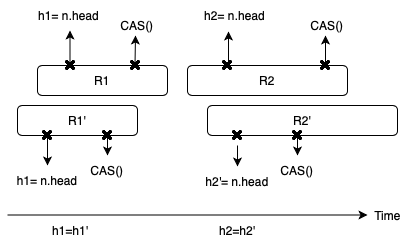
\includegraphics[width=3in]{pics/doublyrefresh.drawio.png}
  \caption{$R_2^\prime$'s \tt{CAS} is executed after \tt{h1=n.head}.}
\end{figure}



  Block \tt{new} is created of new established subblocks of children of \tt{n}(Lemma \ref{lem::createBlock}, Line 46). If \tt{CAS} in Line 48 succeeds then by Lemma~\ref{lem::trueRefresh} new established blocks will be in \tt{n}.
  
\begin{lemma}[Double Refresh] \label{doublyRefresh}
All operations in \tt{n}'s children's blocks before line \tt{35} are guaranteed to be in \tt{n}'s blocks after Line~\tt{37}.
\end{lemma}
%\begin{proof}
%Suppose block \tt{b} with index \tt{i} is in the the left child of \tt{n} before the line 35. By Lemma~\ref{head} it follows that \tt{n.left.head} is greater than \tt{i}. \tt{Refresh()} calls \tt{CreateBlock()} and creates a block from blocks between \tt{n.blocks[n.head].end\textsubscript{left}} and \tt{n.left.head} in the left child, which contains \tt{b} as well. First it tries to append it in \tt{n.blocks.head} and if it was succsuful it continues recursivley. If not it tries again, and if the second call of \tt{Refresh()} in Line 36 fails. It means there is another \tt{Refresh} which has reah its \tt{i} after the Line 35, so it contains \tt{b} as well.
%\end{proof}
\tt{CreateBlock()} reads blocks in the children that do not exist in the parent and aggregates them into one block. If a \tt{Refresh()} procedure returns true it means it has appended the block created by \tt{CreateBlock()} into the parent node's sequence. So suppose two \tt{Refresh}es fail. Since the first \tt{Refresh()} was not successful, it means another CAS operation by a \tt{Refresh}, concurrent to the first \tt{Refresh()}, was successful before the second \tt{Refresh()}. So it means the second failed \tt{Refresh} is concurrent with a successful \tt{Refresh()} that assuredly has read block before the mentioned line \tt{35}. After all it means if any of the \tt{Refresh()} attempts were successful the claim is true, and also if both fail the mentioned claim still holds.

\begin{lemma}[Append]\label{append}
 When \text{\tt{Append(op)}} is finished, \tt{op} appears exactly once in a block of \tt{root.blocks}.
\end{lemma}
%\begin{proof}
%\tt{Append(op)} adds \tt{op} to \tt{l\textsubscript{p}.blocks}(Line~\ref{addOP}) and \tt{Propagate()} recursively propagates \tt{op} up to the root.
%By lemma \ref{doublyRefresh} we know that operation \tt{op} propagates from child to parent at each level.
%\end{proof}

\begin{lemma}[Block Size Upper Bound]\label{blockSize}
Each block in a node contains at most one operation from each processs.  
\end{lemma}
%\begin{proof}
%  Note that \tt{prevIndex} and \tt{lastIndex} defined in lines \ref{lastLine}, \ref{prevLine} are the indices defined in the Definition~\ref{def::subblock}. After a block has propagated to the parent the blocks between \tt{prevIndex} and \tt{lastIndex} make up to the parent (Lemma~\ref{doublyRefresh}). The number of new operations which have not propagated yet to the parent cannot be more than $p$. If so by the law of pigeonholes there is a process which has appended two concurrent operations.
%\end{proof}

\begin{lemma}[Subblocks Upperbound]\label{subBlocksBound}
Each block in a node  has at most $p$ subblocks.
\end{lemma}
%\begin{proof}
%  From Line~\ref{addOP} it is induced directly that each block contains at least one operation. Now it follows directly by Lemma \ref{blockSize}.
%\end{proof}

\begin{definition} [Ordering of operations inside a node] \label{ordering}
$\blacktriangleright$ Note that from Lemma \ref{blockSize} we know there is at most one operation from each process in a given block.

\begin{itemize}
  \item $E(n,i)$ is the sequence of enqueue operations that are member of \tt{n.blocks[i]} ordered by process id.
  \item 
$D(n,i)$ is the sequence of dequeue operations that are member of \tt{n.blocks[i]} ordered by process id.
\item $D(n)=D(n,1).D(n,2).D(n,3)...$
\item $L=E(root,1).D(root,1).E(root,2).D(root,2).E(root,3).D(root,3)...$
\end{itemize}
\end{definition}

\begin{theorem}
The queue implementation is linearizable.
\end{theorem}
%\begin{proof}
%  We show that the ordering $L$ stored in the root, satisfies the properties of a linearizable ordering.
%  \begin{enumerate}
%    \item If $op_1$ ends before $op_2$ begins in $E$, then $op_1$ comes before $op_2$ in $T$.\\$\blacktriangleright$ This is followed by Lemma \ref{append}. The time $op_1$ ends it is in root, before $op_2$, by Definition \ref{ordering} $op_1$ is before $op_2$.
%    \item Responses to operations in $E$ are same as they would be if done sequentially in order of $L$. \\$\blacktriangleright$ Enqueue operations do not have any response so it does no matter how they are ordered. It remains to prove  Dequeue $d$ returns the correct response according to the linearization order. By Lemma \ref{computeHead} it is deduced that the head of the queue at time of the linearization of $d$ is computed properly. If the Queue is not empty by Lemma \ref{get} we know that the returning response is the computed index element.
%  \end{enumerate} 
%\end{proof}

\begin{lemma}[Get] \label{get}
\tt{Get(n,b,i)} returns $i$th Enqueue in $E(n,b)$.
\end{lemma}
%\begin{proof}
%It is obvious that \tt{Get(leaf l,b,1)} returns the operations stored in $b$th block of leaf $l$. To find the \tt{i}th enqueue in block \tt{b} of an internal node \tt{n} in line 87 it is decided that it resides in the left child or the right child. This decision is made by Definition of $E(n,b)$. After that Lines 88, 92 search the proper subblocks of \tt{b}. From Definition~\ref{def::subblock} weknow the subblocks of the $b$th block are within the \tt{prevBlock} and \tt{lastBlock} block of the \tt{CreateBlock()}.
%\end{proof}

\begin{lemma}[Index]
 Index(n,b,i) returns the rank in the $D(root)$ of ith Dequeue in $D(n,b)$.
\end{lemma}
%\begin{proof}
%  \tt{Index(n,b,i)} computes superblock of $i$th Dequeue in $b$th block of \tt{n} in \tt{n.parent} and then computes the order in $D(n.parent, superblock)$. Then calls \tt{index()} on \tt{n.parent} recursively. It is easy to see why the second is correct. Correctness of computing superblock comes from Lemma \ref{superBlock}.
%\end{proof}

\begin{lemma}[Computing SuperBlock]\label{superBlock}
  If \tt{Index(n,b,i)} performs line 101, then \tt{superblock} contains \tt{i}th Dequeue in \tt{b}th block of node \tt{n}.
\end{lemma}
%\begin{proof}
%\begin{enumerate}
% \item Value read for \tt{super[b.time]} in line 101 is not null.\\$\blacktriangleright$
%  Values \tt{c\textsubscript{dir}} read in lines 23, \tt{super} are set before incrementing in lines 26,27.
%
% \item \tt{super[]} preserves order from child to parent; if in a child block \tt{b} is before \tt{c} then \tt{b.time} $\leq$ \tt{c.time} and \tt{super[b.time]} $\leq$ \tt{super[c.time]}\\$\blacktriangleright$
%  Follows from the order of lines 60, 48, 49.
%
%% \item In a propagate step at most 2 different time values are read \\ If there are more than 2 numbers then the smallest number should have been propagated far before.
%% \item There are at most $p^2$ blocks with same time value in a node. \\ At most p processes could die before line 27 and each contains at most p elements.
% \item \tt{super[i+1]-super[i]}$\leq p$
%\\$\blacktriangleright$
% In a Refresh with successful CAS in line 46, \tt{super} and \tt{counter} are set for each child in lines 48,49. Assume the current value of the counter in node \tt{n} is \tt{i+1} and still \tt{super[i+1]} is not set. If an instance of successful \tt{Refresh(n)} finishes \tt{super[i+1]} is set a new value and a block is added after \tt{n.parent[sup[i]]}. There could be at most $p$ successful unfinished concurrent instances of \tt{Refresh()} that have not reached line 49. So the distance between \tt{super[i+1]} and \tt{super[i]} is less than $p$.
%
% \item Superblock of \tt{b} is within range $\pm 2p$ of the \tt{super[b.time]}.
%\\$\blacktriangleright$
%\tt{super[i]} is the index of the superblock of a block containing block b, followed by Lemma \ref{superCounter}. It is trivial to see that \tt{n.super} and \tt{n.b.counter} are increasing. \tt{super(b)} is the real superblock of b. \tt{super(t]} is the index of the superblock of the last block with time \tt{t}. If \tt{b.time} is \tt{t} we have:
%$$super[t]-p\leq super[t-1]\leq super(t-1] \leq super(b) \leq super(t+1)\leq super(t+1]\leq super[t]+p$$
%
%\end{enumerate}
%\end{proof}

\begin{lemma}[Computing Queue's Head] \label{computeHead}
  Let Q be state of the queue if the operations before ith Dequeue in $L(root)$ are applied on the Queue sequentially and X be the head of Q. If Q is empty \tt{ComputeHead(i,b)} returns -1, otherwise
 returns index in $E(root,b)$ of X.
  \end{lemma}

\begin{lemma}[Validity of \tt{head}]\label{head}
No two blocks are written in the same index in \tt{n.blocks}.
\end{lemma}
%\begin{proof}
%  \tt{head} is incremented in lines 51, 54 after trying to append a block to the index of the last \tt{head} read. If it was successful, we have to do this, but if it was unsuccessful, it means it has appended to the index before, so we have to update the \tt{head}. If a process dies before line 51, another process will increment \tt{head} in line 54.
%\end{proof} 

\begin{lemma}[Validity of \tt{super} and \tt{counter}]\label{superCounter}
If \tt{super[i] $\neq$ null}, then \tt{super[i]} in node \tt{n} is the superblock of a block with \tt{time=i}.
\end{lemma}
%\begin{proof}
%After a successful CAS in line 46 \tt{super} and \tt{counter} are modified in both children. \tt{super[i]} is supposed to be the superblock of a block with \tt{time}=i and \tt{counter} is the timer in each node. \tt{super[i]} and \tt{counter=i} are expected to update after a bunch of blocks with \tt{time=i} have been aggregated together into a block in the parent. If the process dies before line 48 these values remain unchanged and incoming blocks will get the same \tt{time}. We claim that our algorithm still works since at most $p$ processes die and it will not change our complexity. If a process dies right after line 48, then \tt{counter} will remain the same and \tt{super[i]} is correct. Furthermore we are sure that when \tt{super[i]} is read it will not be \tt{null}.
%\end{proof}

\begin{lemma}[Search Ranges]\label{search}
  Preconditions of all invocation of \tt{BSearch} are satisfied.
\end{lemma}
%\begin{proof}
%  
%Line 83: \tt{Get(i)} is called if the result of a dequeue is not null. The search is among all blocks in the root.
%
%Line 88: This search tries to find the ith enqueue, knowing that it is in the left child. Search is done over the left subblocks. The start and end of the range are followed by definition. Line 92 is the same.
%
%Line 101: Here, the goal is to find the superblock. We know the distance between answer and the \tt{super[i]} is at most $p$, since at most $p$ processes could die.
%
%\end{proof}


\end{document}






